\documentclass{article}

\usepackage[utf8]{inputenc} 
% \usepackage[swedish]{babel} 
\usepackage{amsmath, amsfonts, amssymb, amsthm}
\usepackage{geometry} 
\usepackage{graphicx} 
\usepackage{hyperref} 
\usepackage{enumerate}
\usepackage{booktabs} 
\usepackage{array}
\usepackage{tikz}
\usepackage{tcolorbox}
\usepackage{pgfplots}
\pgfplotsset{compat=newest}

\geometry{a4paper, margin=1in}


\newtheorem{proposition}{Påstående}
\tcolorboxenvironment{proposition}{
  boxrule=0pt,
  boxsep=2mm,
  colback={orange!10}, % Light orange background
  colframe={orange!50}, % Darker orange frame
  coltitle=blacf(x),
  enhanced,
  sharp corners,
  borderline west={2mm}{0pt}{orange}
}

\title{Ma5 AO5 Omfångsrika problem}
\author{Eduards Abisevs \\ Tetek-21}
\date{\today}

\begin{document}

\maketitle

\section*{Problemformulering}
I en befolkningsmodell för en stor stad kan befolkningstätheten $x$ km från
centrum approximeras med funktionen 
\[
f(x) = \frac{95000}{x^2 + 10x + 16}
\]
där $y$ är antalet människor per kvadratkilometer.

\noindent
\subsection*{Givet}
Av uppgiften ett ledtråd. att teckna ett uttryck.

\noindent
\subsection*{Sökt}
\begin{enumerate}[(a)]
    \item Uppskatta antal människor i en radie 5 km från centrum.
    \item Beräkna antal människor i radie mellan 5 och 10 km.
\end{enumerate}

\begin{proposition}[Modell av befolkningen inom en radie från centrum]
	Given nedre gräns \( a \) och övre gräns \( b \) som tillhör bla bla så gäller modellen: 
	\begin{align*}
		&\int_{a}^{b} \frac{95000 \pi 2 x}{x^2 + 10x + 16} \, dx
		\Rightarrow \\
		&\Rightarrow g(a,b) = \frac{190 000 \pi}{3} \cdot
		\left(4\ln{\left(\frac{|b + 2|}{|a +2|}\right)} 
			-  \ln{\left(\frac{|b + 8|}{|a + 8}\right)} \right)
	\end{align*}
\end{proposition}

\begin{proof}
	HELLO
	\begin{center}

		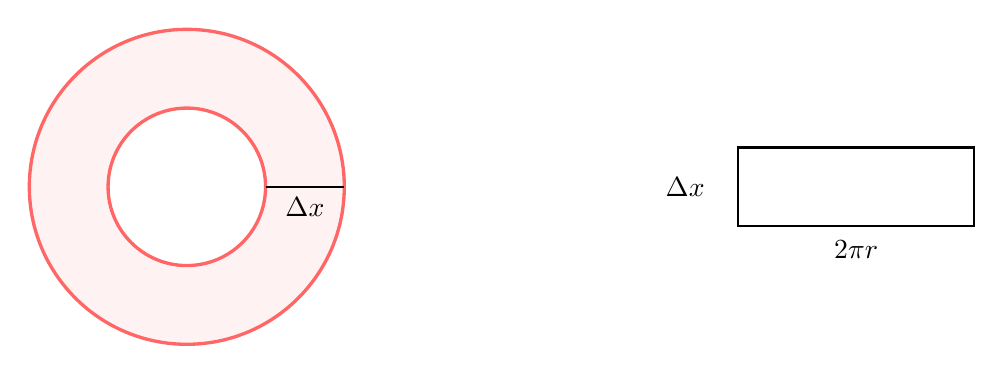
\begin{tikzpicture}
			% Define radii
			\def\rBig{2}
			\def\rSmall{1}

			% Draw the outer circle
			\filldraw[color=red!60, fill=red!5, very thick] (0,0) circle (\rBig);

			% Draw the inner circle
			\filldraw[color=red!60, fill=white, very thick] (0,0) circle (\rSmall);

			% Draw the segment indicating \Delta x
			\draw[thick] (\rSmall,0) -- (\rBig,0) node[midway, below] {$\Delta x$};

			% Calculate middle point for the arrow
			\path (3,0) -- (5,0) coordinate[midway] (midpoint);

			\draw[thick] (7,-\rSmall/2) rectangle (10,\rSmall/2);
			\node at (8.5, -\rSmall/2 - 0.3) {$2\pi\/r$}; 
			\node at (7 - 0.3, 0) [left] {$\Delta x$};  
		\end{tikzpicture}
	\end{center}
	\begin{align*}
		\sum_{a}^{b} \lim_{\Delta x\to 0} \big( f(x) \cdot 2\pi x \cdot \Delta x\big) &=
		\lim_{\Delta x\to 0} \Bigg(\frac{95000 \cdot 2\pi x}{x^2 + 10x + 16} \cdot \Delta x \Bigg)  \\
	\end{align*}
	\begin{align*}
		\int_{a}^{b}{f(x) \, dx }
	\end{align*}
	\end{proof}

\section*{Lösning}
\subsection*{Del (a)}

\subsection*{Del (b)}

\section*{Svar}
\textbf{Del (a)}: \\
\textbf{Del (b)}: 

\end{document}
